
\section{¿Qué es un modelo neuronal?}

En esta sección, se explica qué es un modelo neuronal, sus características y cómo funciona en el contexto de la inteligencia artificial. 

Los modelos neuronales son estructuras computacionales inspiradas en el cerebro humano, diseñadas para procesar información mediante una red de unidades interconectadas que imitan, de manera simplificada, la forma en que las neuronas biológicas se comunican entre sí cite{goodfellow2016deep}.

Los descurbrimientos del Premio Nobel de biología español, Santiago Ramón y Cajal sobre la estructura y funcionamiento de las neuronas, proporcionaron las bases para la comprensión del sistema nervioso en el que se basan los modelos de inteligencia artificial. A finales del siglo XIX, Cajal formuló la teoría de que las neuronas son células individuales conectadas por sinapsis, una idea que revolucionó la neurociencia y sirvió de inspiración para los modelos computacionales de redes neuronales. Su trabajo permitió comprender cómo las señales eléctricas viajan entre las neuronas y cómo se pueden formar conexiones adaptativas, conceptos que más tarde serían adoptados en el diseño de redes neuronales artificiales.

Un modelo neuronal es una arquitectura matemática que busca resolver problemas complejos de aprendizaje mediante el procesamiento de datos. Está compuesto por una serie de unidades de procesamiento, conocidas como neuronas artificiales, organizadas en capas. Cada capa recibe la salida de la capa anterior, aplica una función matemática sobre los datos y transmite el resultado a la siguiente capa. Este proceso se repite de manera secuencial hasta que se alcanza la capa de salida, que proporciona el resultado final del modelo \cite{bishop2006pattern}.

\begin{figure}[H]
    \centering
    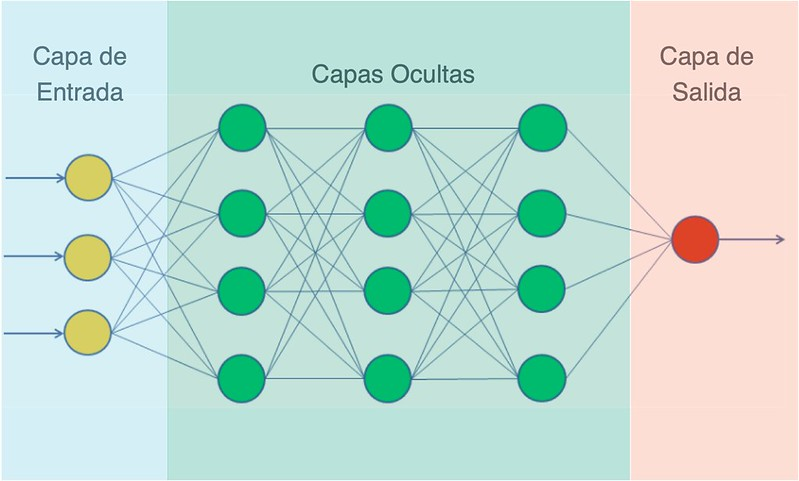
\includegraphics[width=0.8\textwidth]{./img/modelo/capas.png}
    \caption{Esquema de redes neuronales. \cite{aprendeia2021deep}}
    \label{fig:esq-capas}
\end{figure}

Las neuronas dentro de un modelo neuronal no operan de forma aislada, sino que están conectadas entre sí a través de enlaces denominados "pesos". Estos pesos determinan la importancia de la señal que se transmite de una neurona a otra. Durante el proceso de entrenamiento, los pesos se ajustan con el objetivo de minimizar el error en la salida del modelo, lo que permite que el modelo "aprenda" de los datos y mejore su capacidad para predecir o clasificar nueva información \cite{haykin2009neural}.

El proceso de entrenamiento de un modelo neuronal implica la retroalimentación o backpropagation, donde el error de la predicción se calcula y se distribuye hacia atrás a través de la red para ajustar los pesos de manera que el modelo se optimice progresivamente. En este sentido, el modelo neuronal tiene la capacidad de adaptarse a distintos tipos de datos y mejorar su rendimiento con el tiempo \cite{nielsen2015neural}.

A grandes rasgos, un modelo neuronal es una estructura computacional que imita el funcionamiento del cerebro humano para procesar y aprender de datos, y se utiliza en tareas como clasificación, predicción y reconocimiento de patrones.


\subsection{¿Qué tipos de modelos neuronales existen?}

En esta sección se explican cuales son tipos de modelos neuronales existen y sus características principales. 

Los modelos neuronales pueden clasificarse según su estructura, la forma en que procesan la información y la aplicación específica a la que están destinados. Estos modelos neuronales son fundamentales para resolver una variedad de problemas en áreas relacionadas con la inteligencia artificial como la visión por computadora, el procesamiento del lenguaje natural y el reconocimiento de patrones.

Uno de los tipos más comunes de modelos neuronales es el perceptrón multicapa (MLP), que está formado por varias capas de neuronas organizadas en una estructura jerárquica. Cada capa en un MLP recibe la salida de la capa anterior y la procesa mediante una función de activación antes de pasar el resultado a la siguiente capa. Este tipo de red se utiliza principalmente para tareas de clasificación y regresión, y su entrenamiento se realiza utilizando algoritmos como el de retropropagación. Es el tipo de modelo que se utiliza en este proyecto para obtener un modelo capaz de detectar instrusiones en una red informática. \cite{goodfellow2016deep}

Otro tipo importante de modelo neuronal es la red neuronal convolucional (CNN), que está diseñada específicamente para procesar datos con una estructura de cuadricula, como las imágenes. En una CNN, las neuronas están organizadas en capas convolucionales que aplican filtros a los datos de entrada para extraer características relevantes, como bordes, texturas o formas. Esta estructura permite que las CNN sean altamente eficaces para tareas como el reconocimiento de imágenes y la visión por computadora \cite{goodfellow2016deep}.


\begin{figure}[H]
    \centering
    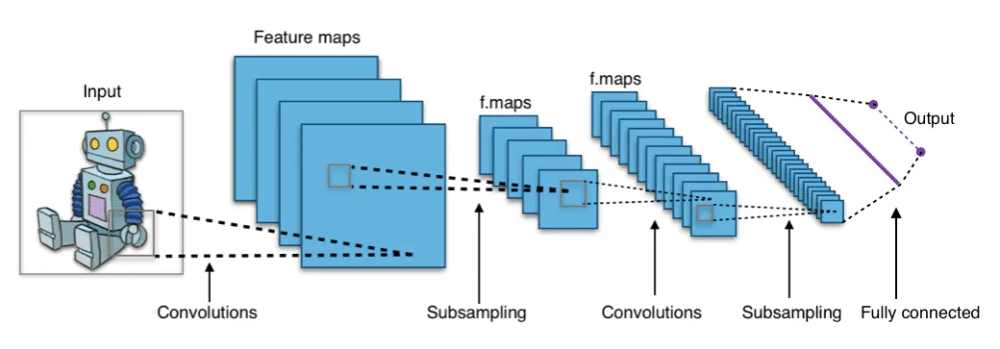
\includegraphics[width=0.8\textwidth]{./img/modelo/CNN.png}
    \caption{Esquema de redes neuronal convolucional. \cite{uniteai2020cnn}}
    \label{fig:esq-CNN}
\end{figure}


Las redes neuronales recurrentes (RNN), por otro lado, son adecuadas para procesar secuencias de datos, como el texto o el audio. Las RNN son únicas porque sus neuronas tienen conexiones que permiten que la información fluya hacia atrás a lo largo del tiempo, lo que las hace útiles para modelar dependencias temporales en los datos. Este tipo de red es comúnmente utilizado en tareas de procesamiento de lenguaje natural y en modelos de predicción de series temporales \cite{haykin2009neural}.

En un enfoque más avanzado, existen las redes generativas antagónicas (GAN), que se componen de dos redes neuronales: un generador y un discriminador. El generador crea datos falsos a partir de ruido, mientras que el discriminador intenta diferenciar entre los datos reales y los generados. A través de un proceso de entrenamiento competitivo, ambas redes mejoran en sus respectivas tareas. Las GANs se utilizan principalmente en la generación de imágenes, música y otros tipos de contenido artístico \cite{nielsen2015neural}.

\subsection{Función de perdida}
En esta sección se explica que es una función de pérdida y su importancia en el proceso de entrenamiento de un modelo neuronal. También se justifica el uso de las funciones de pérdida que se emplean para el entrenamiento de los modelos de este trabajo.

Una función de pérdida es un componente fundamental en el entrenamiento de modelos de aprendizaje automático, cuya finalidad consiste en cuantificar la discrepancia entre las predicciones generadas por el modelo y los valores reales esperados. Esta medida permite guiar el proceso de optimización, ya que el objetivo durante el entrenamiento es minimizar dicha pérdida para mejorar la precisión del modelo.\cite{eitca_loss_function}

Las funciones de pérdida desempeñan un papel central en la formulación matemática del aprendizaje supervisado, al establecer una métrica que penaliza el error cometido por el modelo. Esta penalización permite que los algoritmos de optimización, como el descenso por gradiente, ajusten iterativamente los parámetros del modelo en la dirección que reduce la pérdida total. Para que esta estrategia sea efectiva, la función de pérdida debe poseer ciertas propiedades fundamentales:

\begin{itemize}

    \item\textbf{Diferenciabilidad}: Permite el cálculo de gradientes necesarios para optimizar los parámetros mediante técnicas basadas en derivadas, como el descenso por gradiente.

    \item\textbf{Convexidad (deseable)}: Favorece la convergencia hacia un mínimo global, aunque en la práctica, muchos modelos no lineales presentan funciones de pérdida no convexas.

    \item\textbf{Estabilidad numérica}: Previene errores computacionales al manejar valores extremos o transformaciones exponenciales, manteniendo precisión durante el entrenamiento.

 	\item\textbf{Sensibilidad al error}: Garantiza que los errores mayores se penalicen de forma más significativa, orientando el modelo hacia mejores predicciones.

	\item\textbf{Escalabilidad}: Permite su aplicación eficiente en contextos con grandes volúmenes de datos y arquitecturas de red complejas.

\end{itemize}

Estas propiedades aseguran que la función de pérdida cumpla su objetivo central, actuar como un mecanismo confiable y eficiente para guiar la actualización de los parámetros del modelo. \cite{ultralytics_loss_function}

En el caso específico del modelo de clasificación binaria, se opta por la función BCEWithLogitsLoss (Binary Cross Entropy with Logits Loss), que está especialmente recomendada para utilizarse en entornos de aprendizaje profundo como PyTorch, entorno utilizado en el desarrollo práctico de este proyecto. Esta función combina en una sola operación dos pasos fundamentales: la aplicación de la función sigmoide y el cálculo de la entropía cruzada binaria. Al integrar ambos procedimientos en una única función, se obtienen varias ventajas prácticas.\cite{datacamp_loss_function}

En primer lugar, se mejora la estabilidad numérica, ya que evita operaciones redundantes que podrían dar lugar a pérdidas de precisión, especialmente al manejar las salidas no normalizadas del modelo (logits) con valores extremos.

En segundo lugar, se optimiza el rendimiento computacional, al reducir el número de transformaciones necesarias antes del cálculo de la pérdida. 

Finalmente, permite trabajar directamente con logits, lo cual simplifica la implementación y reduce errores potenciales derivados de transformaciones incorrectas. \cite{bigdatafran_pytorch_classification}




\subsection{Algoritmo de optimización}


\section{Modelo neuronal de clasificación binaria}
\section{Modelo neuronal de clasificación multiclase}

\section{Métricas}  \label{sec.metricas}
\subsection{Matriz de confusión} \label{sec.matriz-consfusion}
En esta sección se explica en que consiste una matriz de confusión. Una matriz de confusión es una herramienta fundamental utilizada en el campo del aprendizaje automático y la clasificación, especialmente cuando se evalúan modelos de clasificación como el que se propone en este proyecto.


La matriz de confusión es una representación tabular que permite evaluar el rendimiento de un modelo de clasificación. Esta matriz compara las predicciones del modelo con los valores reales (verdaderos) y proporciona una visión detallada sobre los errores cometidos. Esta matriz permite calcular diversas métricas de evaluación del modelo, que son esenciales para entender la efectividad del modelo en tareas de clasificación.

En el caso de los modelos neuronales de clasificación binaria, la matriz tiene una estructura 2x2, donde cada celda en la matriz representa la cantidad de veces que una combinación específica de clase real y clase predicha ocurrió. Los valores posibles para la clasificación binaria son: 

\begin{itemize}

	\item Verdaderos positivos (VP): son las instancias que pertenecen a la clase positiva y que el modelo ha clasificado correctamente como positivas.

    \item Falsos positivos (FP): corresponden a las instancias que no pertenecen a la clase positiva, pero que el modelo ha etiquetado incorrectamente como positivas.

    \item Falsos negativos (FN): se refieren a las instancias que deberían ser clasificadas como positivas, pero que el modelo ha predicho como negativas.

    \item Verdaderos negativos (VN): son las instancias que pertenecen a la clase negativa y que el modelo ha clasificado correctamente como negativas.

\end{itemize}



\begin{table}[h]
\centering
\label{tab:confusion_matrix}
\begin{tabular}{|l|c|c|}
\hline
 & \textbf{Predicción Positiva} & \textbf{Predicción Negativa} \\ \hline
\textbf{Real Positivo} & Verdaderos Positivos (VP) & Falsos Negativos (FN) \\ \hline
\textbf{Real Negativo} & Falsos Positivos (FP) & Verdaderos Negativos (VN) \\ \hline
\end{tabular}
\caption{Matriz de confusión para clasificación binaria.}
\end{table}


Para un modelo con múltiples clases, como el caso de un modelo neuronal con 9 salidas, la matriz tiene las siguientes interpretaciones:
\begin{itemize}
	\item Diagonal principal: Cada celda de la diagonal principal de la matriz representa cuántas veces la clase real fue correctamente predicha como clase. Este es el caso de las instancias que fueron correctamente clasificadas, y es lo más cercano a un "verdadero positivo" para esa clase específica. Sin embargo, en clasificación multiclase, se suele hablar de "aciertos" o "instancias correctamente clasificadas" para cada clase.

	\item Fuera de la diagonal: Las celdas fuera de la diagonal representan falsas clasificaciones. Es decir, representan cuántas veces una instancia de la clase real fue predicha incorrectamente como otra clase.

\end{itemize}


\begin{table}[h]
\centering
\label{tab:confusion_matrix_9class}
\resizebox{\textwidth}{!}{
\begin{tabular}{|l|c|c|c|c|c|c|c|c|c|}
\hline
 & \textbf{Predicción Clase 1} & \textbf{Predicción Clase 2} & \textbf{Predicción Clase 3} & \textbf{Predicción Clase 4} & \textbf{Predicción Clase 5} & \textbf{Predicción Clase 6} & \textbf{Predicción Clase 7} & \textbf{Predicción Clase 8} & \textbf{Predicción Clase 9} \\ \hline
\textbf{Real Clase 1} & VP$_{1}$ & FP$_{12}$ & FP$_{13}$ & FP$_{14}$ & FP$_{15}$ & FP$_{16}$ & FP$_{17}$ & FP$_{18}$ & FP$_{19}$ \\ \hline
\textbf{Real Clase 2} & FP$_{21}$ & VP$_{2}$ & FP$_{23}$ & FP$_{24}$ & FP$_{25}$ & FP$_{26}$ & FP$_{27}$ & FP$_{28}$ & FP$_{29}$ \\ \hline
\textbf{Real Clase 3} & FP$_{31}$ & FP$_{32}$ & VP$_{3}$ & FP$_{34}$ & FP$_{35}$ & FP$_{36}$ & FP$_{37}$ & FP$_{38}$ & FP$_{39}$ \\ \hline
\textbf{Real Clase 4} & FP$_{41}$ & FP$_{42}$ & FP$_{43}$ & VP$_{4}$ & FP$_{45}$ & FP$_{46}$ & FP$_{47}$ & FP$_{48}$ & FP$_{49}$ \\ \hline
\textbf{Real Clase 5} & FP$_{51}$ & FP$_{52}$ & FP$_{53}$ & FP$_{54}$ & VP$_{5}$ & FP$_{56}$ & FP$_{57}$ & FP$_{58}$ & FP$_{59}$ \\ \hline
\textbf{Real Clase 6} & FP$_{61}$ & FP$_{62}$ & FP$_{63}$ & FP$_{64}$ & FP$_{65}$ & VP$_{6}$ & FP$_{67}$ & FP$_{68}$ & FP$_{69}$ \\ \hline
\textbf{Real Clase 7} & FP$_{71}$ & FP$_{72}$ & FP$_{73}$ & FP$_{74}$ & FP$_{75}$ & FP$_{76}$ & VP$_{7}$ & FP$_{78}$ & FP$_{79}$ \\ \hline
\textbf{Real Clase 8} & FP$_{81}$ & FP$_{82}$ & FP$_{83}$ & FP$_{84}$ & FP$_{85}$ & FP$_{86}$ & FP$_{87}$ & VP$_{8}$ & FP$_{89}$ \\ \hline
\textbf{Real Clase 9} & FP$_{91}$ & FP$_{92}$ & FP$_{93}$ & FP$_{94}$ & FP$_{95}$ & FP$_{96}$ & FP$_{97}$ & FP$_{98}$ & VP$_{9}$ \\ \hline
\end{tabular}
}
\caption{Matriz de confusión para clasificación con 9 clases.}
\end{table}


\subsection{Fórmulas e Interpretación}


Para evaluar el desempeño del modelo de detección y clasificación de ataques, se utilizan las siguientes métricas derivadas de la matriz de confusión.


\begin{itemize}
    \item \textbf{Exactitud (\textit{Accuracy})}: \label{met:Accuracy}
    
\begin{equation}
    \text{Accuracy} = \frac{VP + VN}{VP + FP + VN + FN}
\end{equation}

En el entrenamiento de modelos neuronales para la detección de intrusiones, esta métrica representa la proporción del total de las clasificaciones realizadas correctamente. Indica la capacidad general del modelo para distinguir entre tráfico normal e intrusivo. Si bien ofrece una visión global del rendimiento, su valor disminuye en escenarios donde la cantidad de tráfico normal supera significativamente al tráfico malicioso, ya que el modelo puede obtener una alta exactitud simplemente clasificando la mayoría de las instancias como normales.

\item \textbf{Precisión (\textit{Precision})}: \label{met:Precision}

\begin{equation}
    \text{Precision} = \frac{VP}{VP + FP}
\end{equation}

Esta métrica evalúa la capacidad del modelo neuronal para evitar la identificación incorrecta de tráfico normal como intrusivo. En la detección de intrusiones, una alta precisión es crucial para minimizar las falsas alarmas, las cuales pueden generar una sobrecarga operativa en los equipos de seguridad, requiriendo la revisión de eventos benignos y distrayendo la atención de amenazas reales. Un modelo preciso reduce la fatiga de alertas y permite una respuesta más eficiente a incidentes genuinos.

\item \textbf{Sensibilidad (\textit{Recall})}: \label{met:Recall}

\begin{equation}
    \text{Recall} = \frac{VP}{VP + FN}
\end{equation}

La sensibilidad mide la habilidad del modelo neuronal para detectar todas las instancias de intrusión presentes en el tráfico de red. En el contexto de la seguridad, un alto recall es de suma importancia, ya que implica una menor probabilidad de que ataques reales pasen desapercibidos. Un modelo con baja sensibilidad puede tener consecuencias graves, permitiendo que actividades maliciosas se infiltren y comprometan la integridad y la confidencialidad de los sistemas.

\item \textbf{Puntuación F1 (\textit{F1-Score})}: \label{met:F1-score}

\begin{equation}
    F1 = 2 \times \frac{\text{Precision} \times \text{Recall}}{\text{Precision} + \text{Recall}}
\end{equation}

Esta métrica proporciona una evaluación equilibrada del rendimiento del modelo neuronal al calcular la media armónica entre la precisión y el recall. En la detección de intrusiones, donde a menudo existe un desequilibrio entre el tráfico normal y el malicioso, el F1-score ofrece una métrica más robusta que la exactitud, ya que considera tanto la capacidad de evitar falsas alarmas como la de detectar todas las intrusiones. Un valor alto de F1-score indica un buen compromiso entre ambas capacidades.

\item \textbf{Puntuación F2 (\textit{F2-Score})}: \label{met:F2-score}

\begin{equation}
    F2 = 5 \times \frac{\text{Precision} \times \text{Recall}}{4 \times \text{Precision} + \text{Recall}}
\end{equation}

Esta variante de la puntuación F pondera la sensibilidad más que la precisión. En el ámbito de la detección de intrusiones, el F2-score resulta útil cuando las consecuencias de no detectar un ataque (falso negativo) se consideran significativamente más perjudiciales que generar una falsa alarma (falso positivo). Al asignar un mayor peso al recall, se prioriza la identificación de la mayor cantidad posible de actividades maliciosas, incluso a expensas de un posible aumento en las falsas alertas.
\end{itemize}


\subsection{Aplicación en Seguridad}	\label{sec:apli-met-seg}
En el contexto de detección de intrusiones:
\begin{itemize}
    \item Un recall alto (> 95\%) asegura que pocos ataques pasan desapercibidos.
    \item La precisión debe optimizarse para reducir la carga operativa de analistas (falsos positivos < 10\%).
    \item El F2-Score es preferible al F1 cuando la prioridad es minimizar riesgos de ataques no detectados.
\end{itemize}
